\chapter{Evaluation}
\label{cha:evaluation}

This chapter reports the depth comparison and qualitative pipeline results. The looser
self-collected videos have no depth ground truth, so most measures here address stability and
geometry preservation rather than accuracy.

\section{Evaluation Setup and Datasets}
\label{sec:eval-setup}

The evaluation uses PhysTwin's released RGBD data \parencite{phystwin} and about 30 self-collected
multi-view sessions of cloth, mats, bottles, mugs and stuffed animals; an earlier batch contained
about eight sessions. The first rig used two phones and a DJI action camera, with different
intrinsics, rolling shutters, auto-exposure and autofocus. The cameras were not time-synchronised.
The later rig recorded colour and depth with three Intel RealSense D415 cameras and measured the
intrinsics and extrinsics manually as a reference, although the pipeline still infers poses; those sessions carry a metric depth reference, and the earlier
batch has none.


\section{Measuring Depth Quality Without Ground Truth}
\label{sec:eval-protocol}

A depth error can only be measured against a sensor reference. PhysTwin's released sequences and
the stricter self-collected sessions both carry sensor depth, but it is sparse and noisy relative to
the dense predictions, and the looser-protocol videos have no reference at all. The evaluation
therefore reports one relative comparison against the sensor
(Section~\ref{sec:eval-depth-sensor}), covering a single sequence, and treats the rest
qualitatively: flicker removal (Section~\ref{sec:eval-depth-cases}), tracking
(Section~\ref{sec:eval-tracking}) and the end-to-end results. Each result is only a proxy, because
smoothing can reduce flicker while flattening or blurring geometry. There are no cross-view or
warp-model scores, and no quantitative VDA or streaming-baseline comparison. End-to-end findings
below are the author's own visual judgement. No other raters scored them, and no formal rating protocol was used. No loss-term ablation
or temporal-span sweep was performed; their effects and weight sensitivity remain
unmeasured.\label{sec:eval-ablations}


\section{Depth against the sensor reference}
\label{sec:eval-depth-sensor}
\label{sec:eval-depth}

PhysTwin's released sequences carry RealSense depth, as do the stricter self-collected sessions,
which were recorded with three RealSense D415 cameras capturing colour and depth together. The
comparison below uses the released double-stretch sloth sequence: the raw inferred depth and the
smoothed depth were each compared with the sensor reference over all 192 frames of the three
cameras (\texttt{evaluation/compare\_depth.py}).
The comparison measures relative depth: Spearman rank correlation of the depth ordering, Pearson
correlation of Sobel gradient magnitudes, the ordinal error (the fraction of sampled point pairs
whose ordering is reversed), and the scale-invariant RMSE after a
least-squares scale-and-shift alignment. The sensor depth is sparse and noisy around object
boundaries, which limits all four measures.

\begin{figure}[H]
	\begin{center}
		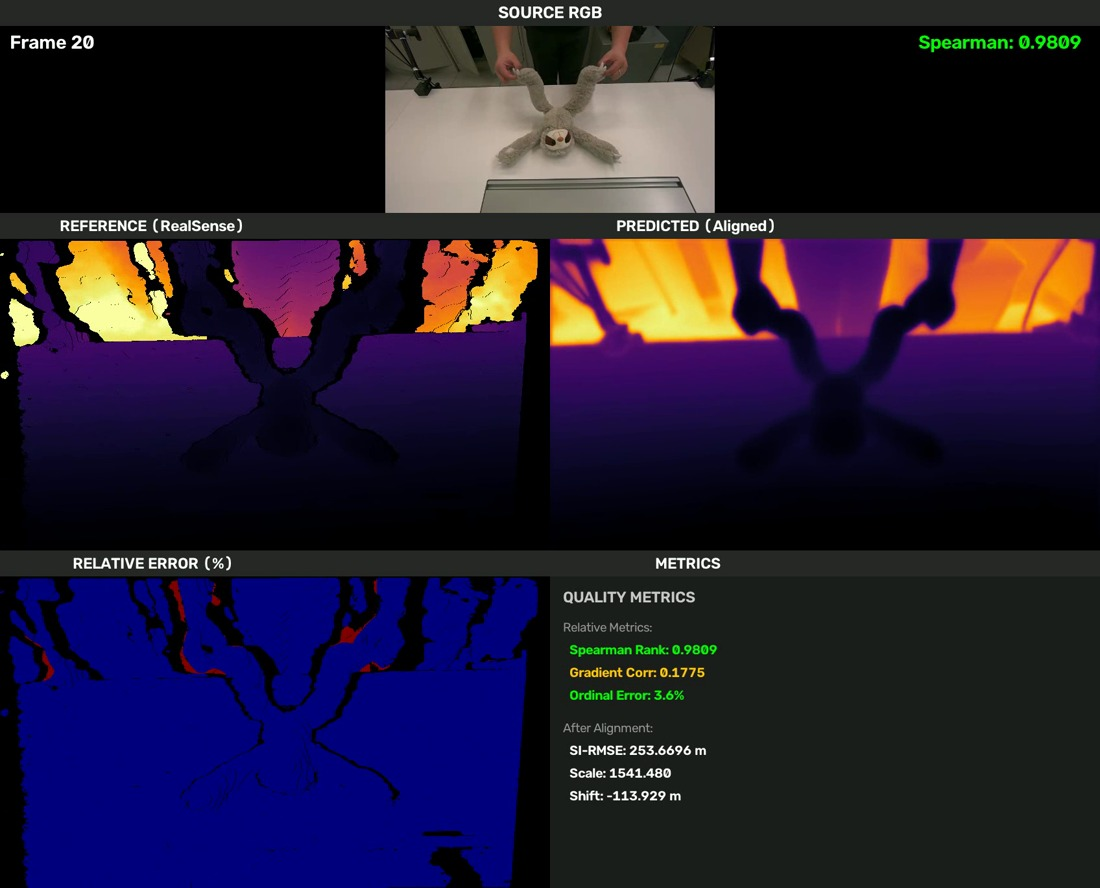
\includegraphics[width = \textwidth]{Images/depth_vs_sensor}
		\caption{One frame (20 of 192) of the sloth sequence after smoothing: source RGB, RealSense
		reference depth, aligned smoothed depth, error map and per-frame metrics.}
		\label{fig:eval-depth-sensor}
	\end{center}
\end{figure}

\begin{table}[H]
    \caption{Relative depth quality against the RealSense reference over 192 frames of the
    double-stretch sloth sequence, per camera, for the raw inferred depth (top) and the smoothed
    depth (bottom). SI-RMSE is in millimetres after scale-and-shift alignment.}
    \label{tab:eval-depth-sensor}
    \begin{center}
        \small
        \begin{tabular}{@{}llcccc@{}}
            \toprule
            Depth & Camera & Spearman $\uparrow$ & Gradient corr.\ $\uparrow$ & Ordinal error $\downarrow$ & SI-RMSE $\downarrow$ \\
            \midrule
            Raw DA3 & 0 & 0.988 & 0.117 & 3.3\% & 346 \\
                    & 1 & 0.945 & 0.115 & 6.9\% & 666 \\
                    & 2 & 0.963 & 0.090 & 4.2\% & 1495 \\
            \midrule
            Smoothed & 0 & 0.988 & 0.169 & 3.3\% & 343 \\
                     & 1 & 0.951 & 0.151 & 6.6\% & 664 \\
                     & 2 & 0.964 & 0.122 & 4.5\% & 1494 \\
            \bottomrule
        \end{tabular}
    \end{center}
\end{table}

The depth ordering is nearly perfect for both variants and few point pairs are misordered. Smoothing
leaves the ordering and the aligned error almost unchanged and raises the gradient correlation on every
camera (0.107 to 0.147 on average), so the smoothed depth still agrees with the sensor
reference. On camera 0 the per-frame ordinal error varies little (2.3--4.6\%, median 3.25\%): most
sampled pairs span large depth differences, which both variants order correctly, while the errors
concentrate on near-tie pairs within the object and at its boundary. The gradient correlation is
still modest: local depth structure remains weaker than the
sensor's, which matches the inconsistent boundaries observed in Section~\ref{sec:design-depth}. The
measurement covers one sequence and compares the inferred depth with the sensor; it does not compare
the four depth sources end to end.

\begin{figure}[H]
	\begin{center}
		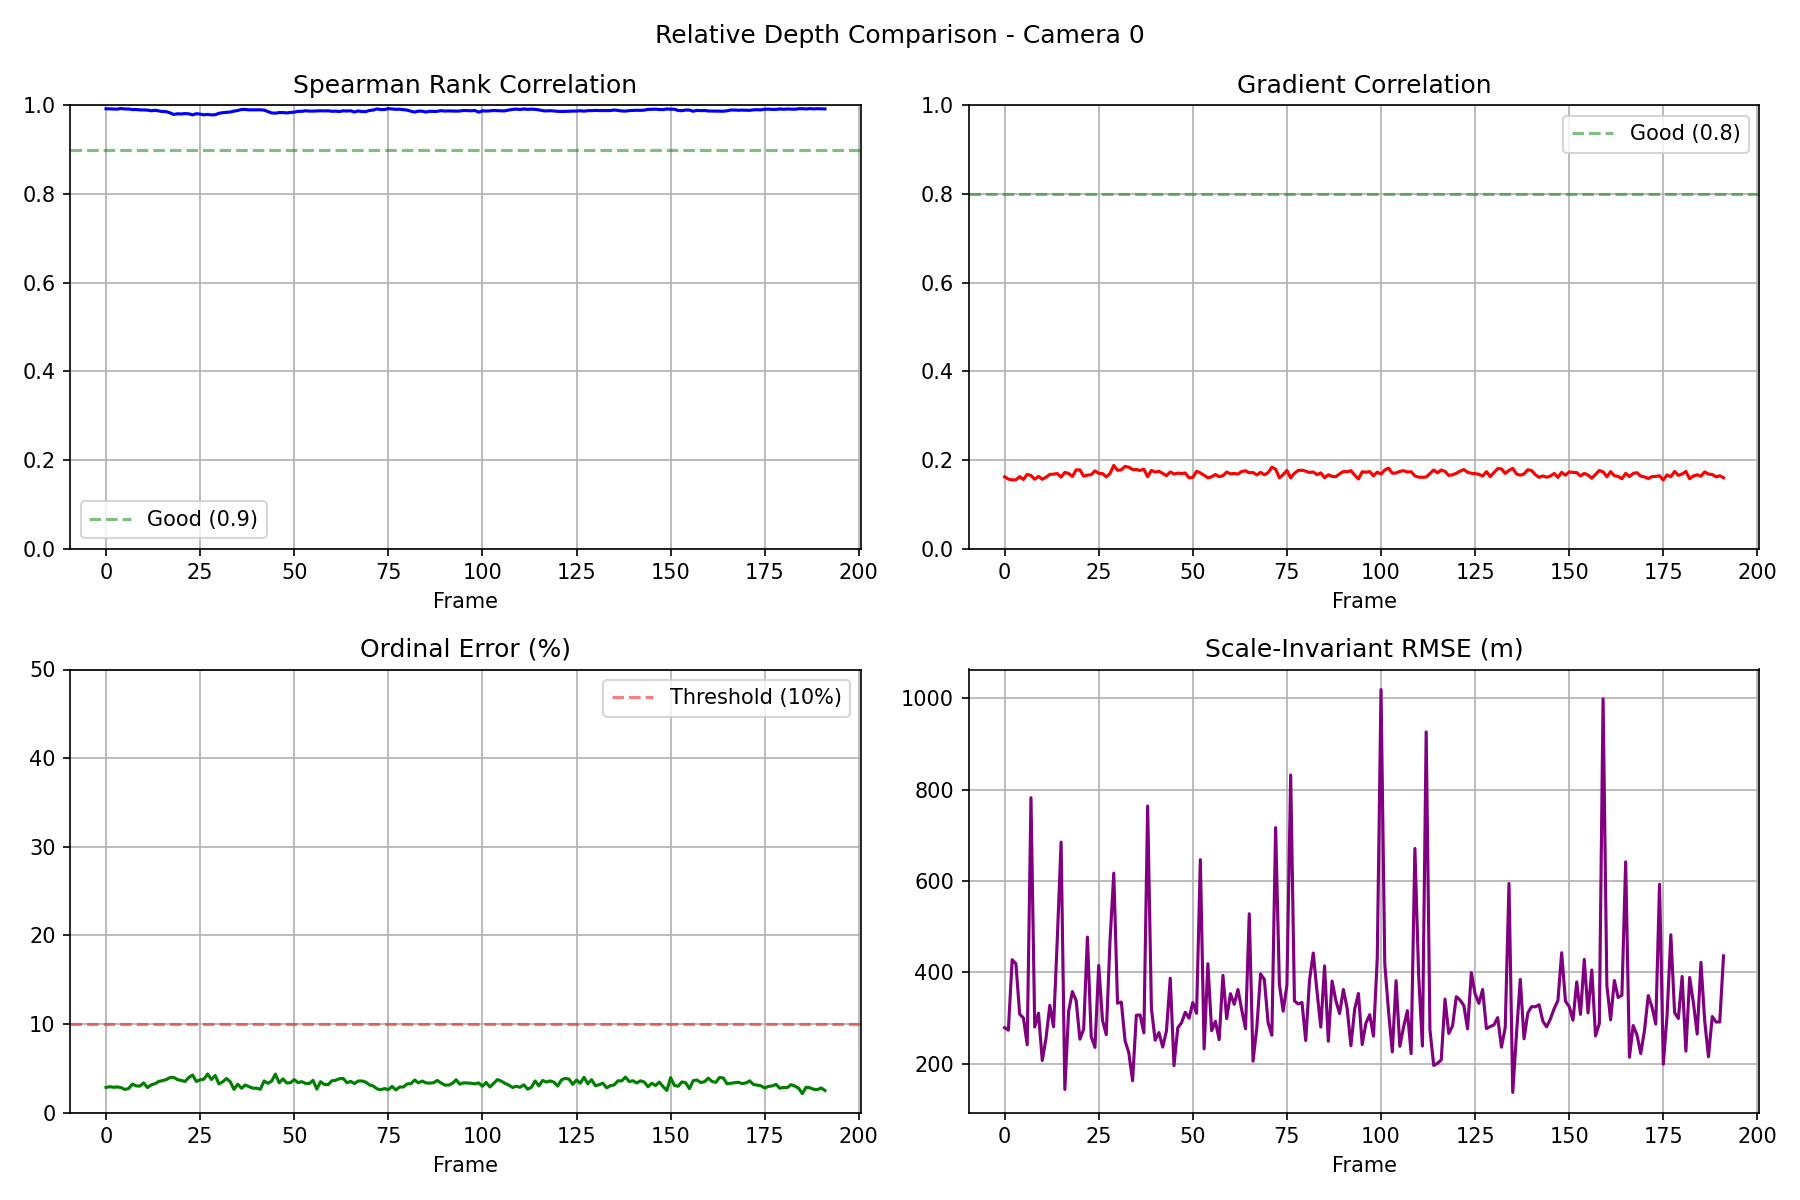
\includegraphics[width = 0.85\textwidth]{Images/depth_quality_metrics}
		\caption{Per-frame relative depth metrics for the smoothed depth, camera 0: Spearman rank
		correlation, gradient correlation, ordinal error and SI-RMSE.}
		\label{fig:eval-depth-metrics}
	\end{center}
\end{figure}

\section{Flicker removal across sequences}
\label{sec:eval-depth-cases}

Figures~\ref{fig:eval-depth-cases} and~\ref{fig:eval-depth-cases-2} show five consecutive frames
of five sequences, raw DA3 above and smoothed below, with a shared colour scale per sequence. In the
raw rows the depth of static surfaces shifts from frame to frame and the object--background boundary
moves; the smoothed rows are stable frame to frame at the cost of softer boundaries. The smoothed
rows come from the best saved model,
\texttt{best\_model\_50\_epochs\_no\_edge\_blur}. Sequences include sloth, monkey, mat, rope and
cloth; the monkey and mat rows use looser-protocol captures. Video recordings of the raw
and smoothed depth are listed in Appendix~\ref{sec:app-vid-smoother}, and pipeline replays before and
after smoothing in Appendix~\ref{sec:app-vid-smoother}.

\begin{figure}[H]
	\begin{center}
		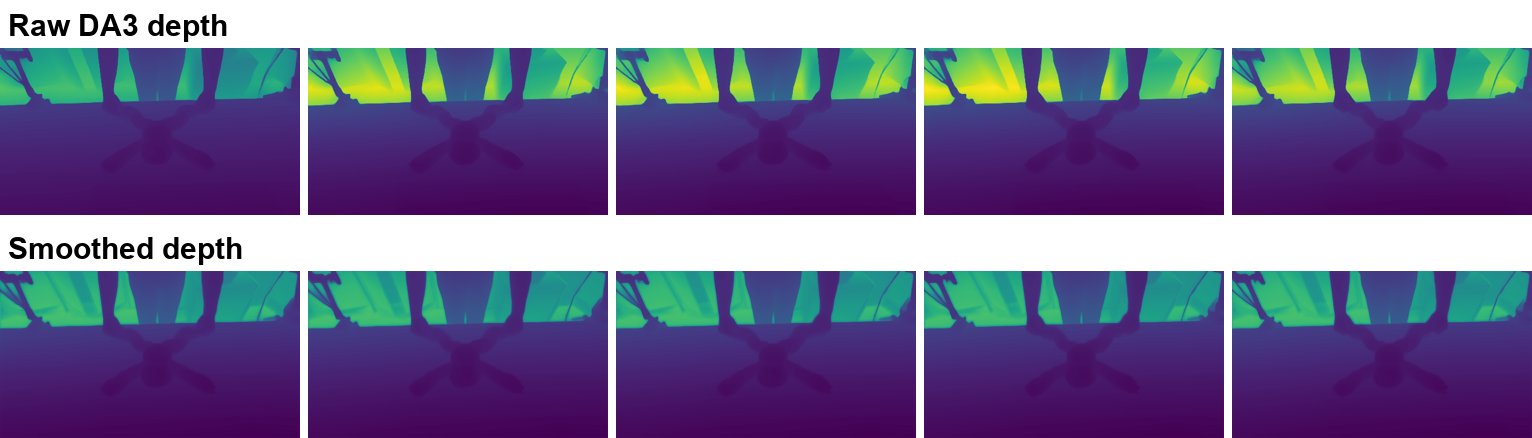
\includegraphics[width = \textwidth]{Images/depth_case_sloth}\\
		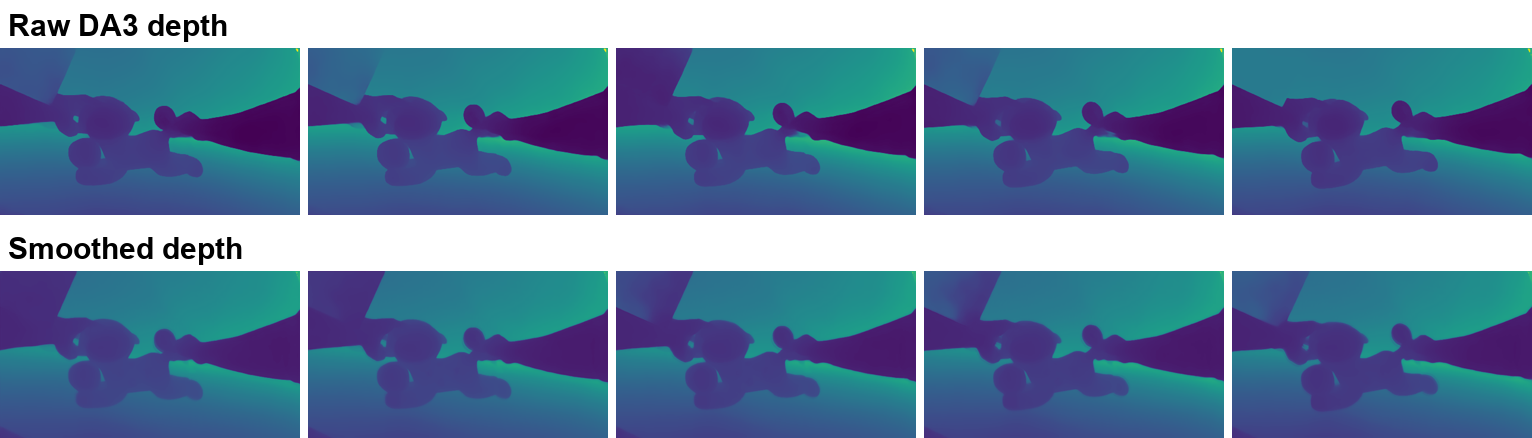
\includegraphics[width = \textwidth]{Images/depth_case_monkey}\\
		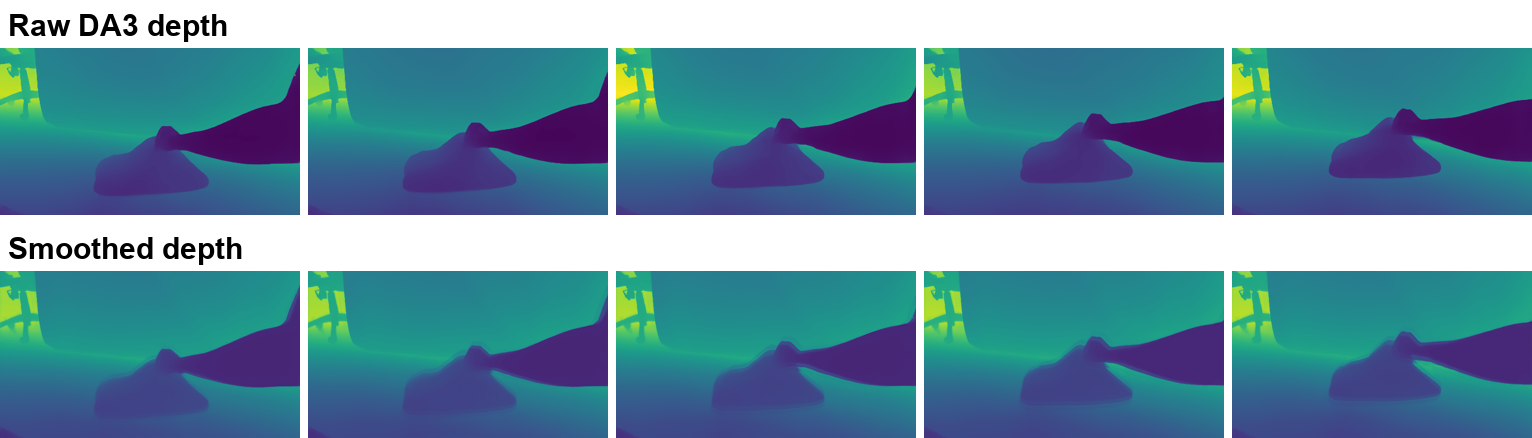
\includegraphics[width = \textwidth]{Images/depth_case_pad}
		\caption{Raw DA3 (top) and smoothed depth (bottom) for five consecutive frames of each
		sequence: sloth stretch, monkey bend and mat lift.}
		\label{fig:eval-depth-cases}
	\end{center}
\end{figure}

\begin{figure}[H]
	\begin{center}
		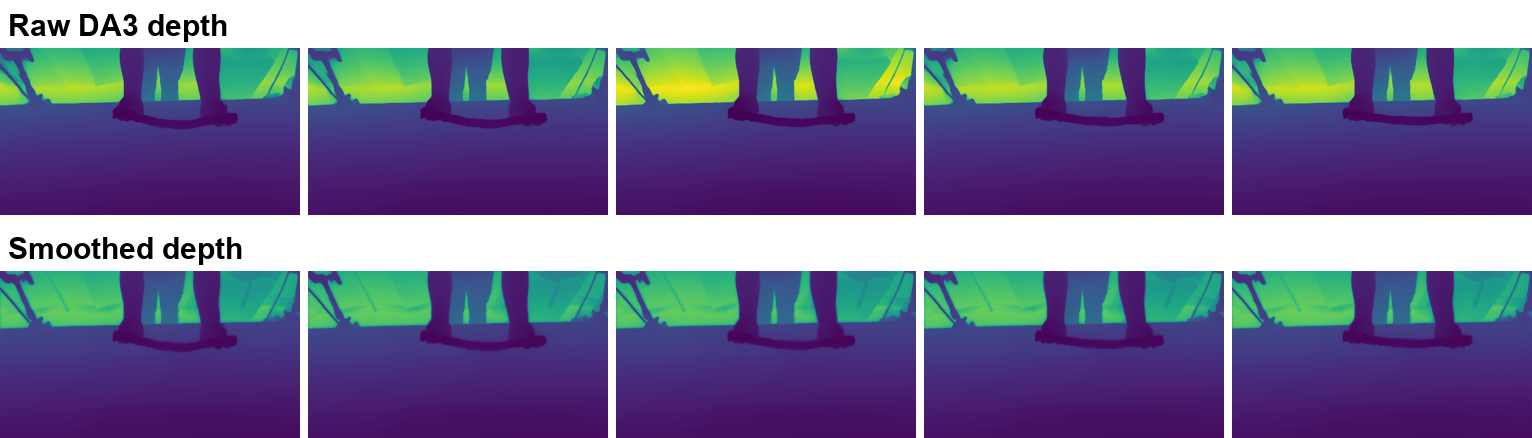
\includegraphics[width = \textwidth]{Images/depth_case_rope}\\
		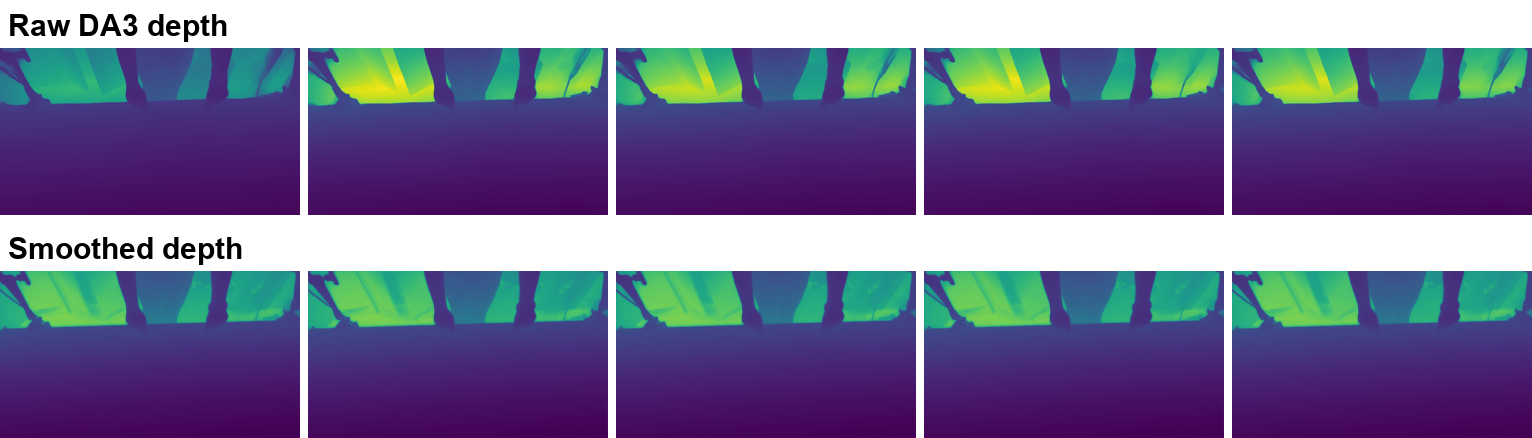
\includegraphics[width = \textwidth]{Images/depth_case_cloth}
		\caption{The same comparison for the rope and cloth sequences.}
		\label{fig:eval-depth-cases-2}
	\end{center}
\end{figure}

\section{Effect on Tracking}
\label{sec:eval-tracking}

The track comparisons ask how much the recovered 3D tracks change between pipeline
variants. Each pair of runs reconstructs the same sequence from differently built input data: either
the depth source differs (the original sensor depth and the new inferred depth), or only the temporal
smoothing of the inferred depth differs. The comparison scripts did not isolate these factors
reliably and reported differences that are not physically plausible: tens of centimetres of
trajectory error between runs whose inputs differ only in the depth treatment. Those figures are
therefore not reported here. The effect of the depth source itself is compared qualitatively in
Section~\ref{sec:eval-ognew}, and the cloth pair below is the clearest example of the effect of
smoothing.

Figure~\ref{fig:eval-track-vis} visualises that cloth pair
(\texttt{single\_lift\_cloth\_3\_new} against \texttt{single\_lift\_cloth\_3\_smooth}), which
differs only in whether the inferred depth was smoothed. The tracked object points of the two runs
overlap almost completely, and the spread and velocity curves show that smoothing the inferred
depth removes frame-to-frame jitter while the recovered motion is preserved.

\begin{figure}[H]
	\begin{center}
		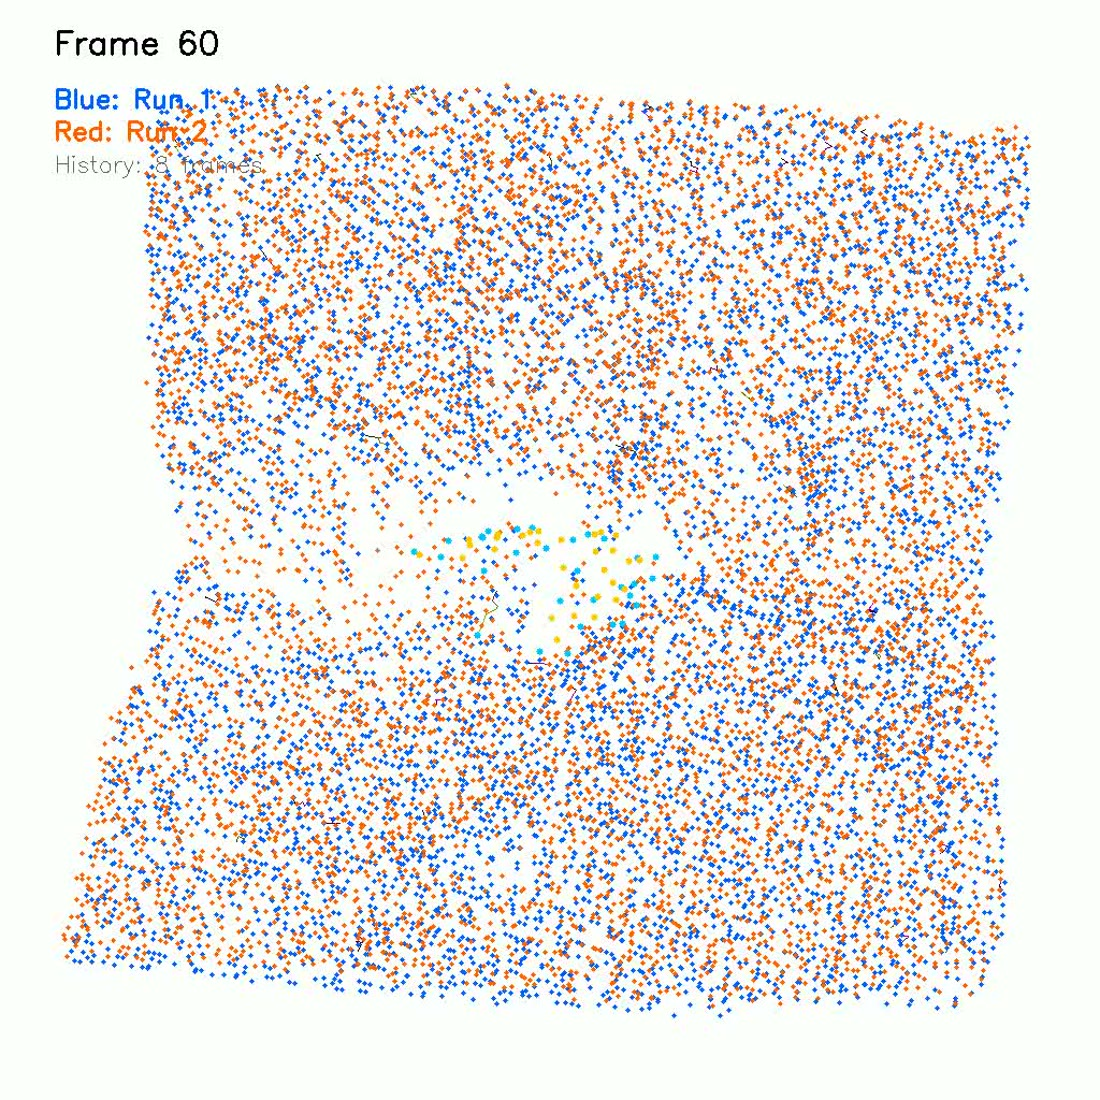
\includegraphics[width = 0.72\textwidth]{Images/track_overlay_ghosts}\\
		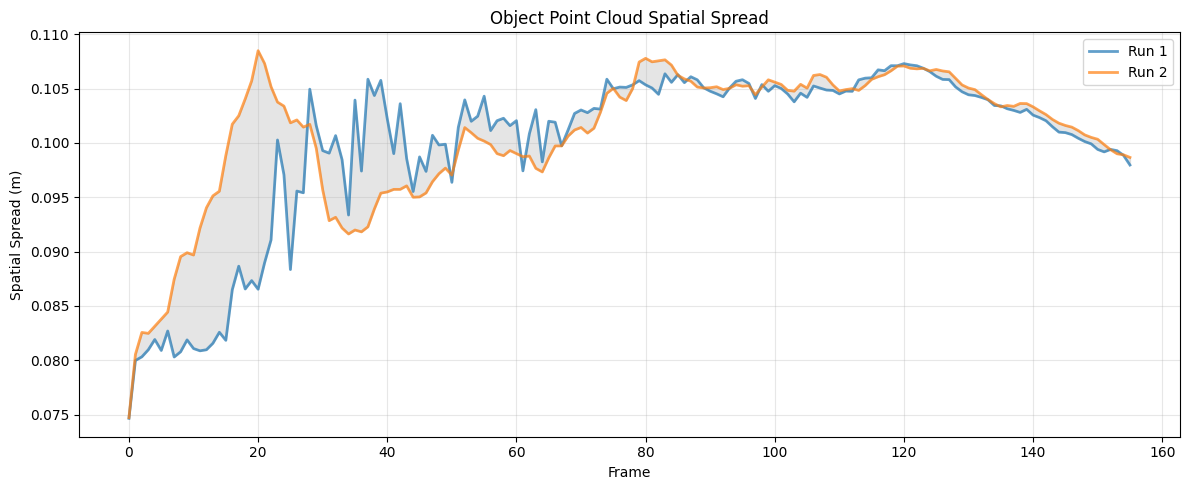
\includegraphics[width = 0.48\textwidth]{Images/track_object_spread}\hfill
		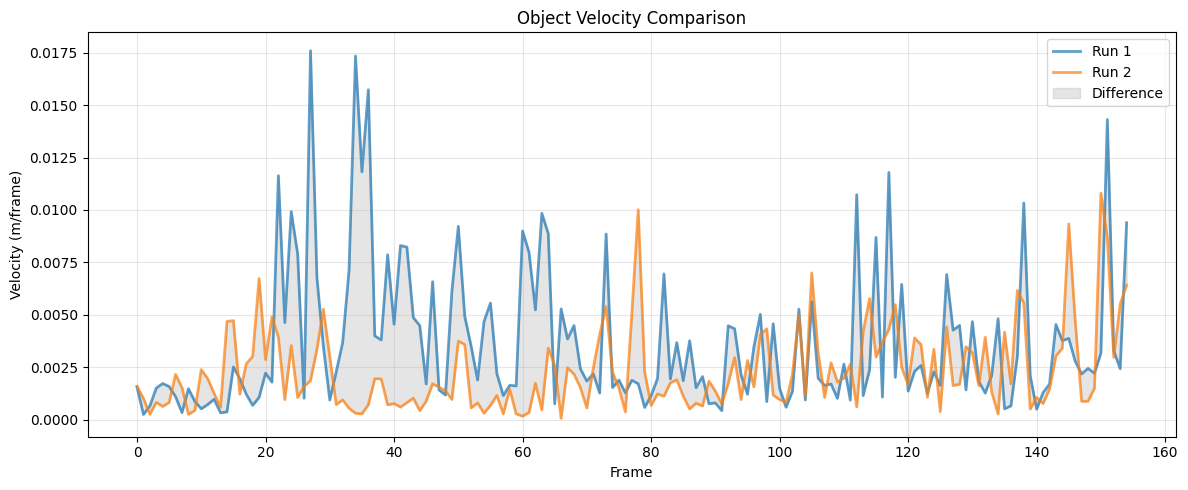
\includegraphics[width = 0.48\textwidth]{Images/track_object_velocity}
		\caption{Tracking for the cloth pair (\texttt{single\_lift\_cloth\_3\_new} against
		\texttt{single\_lift\_cloth\_3\_smooth}). Top: tracked points of both runs overlaid.
		Bottom: object point-cloud spread and velocity; Run 1 unsmoothed, Run 2 smoothed.}
		\label{fig:eval-track-vis}
	\end{center}
\end{figure}

\section{End-to-End Results}
\label{sec:eval-endtoend}

DIPhysTwin completed on PhysTwin and self-collected data and produced interactive spring--mass
warp models. On PhysTwin sequences, the author's visual inspection found the results broadly similar to the RGBD baseline.
All runs use inferred poses, depth and ground alignment.

\begin{figure}[H]
	\begin{center}
		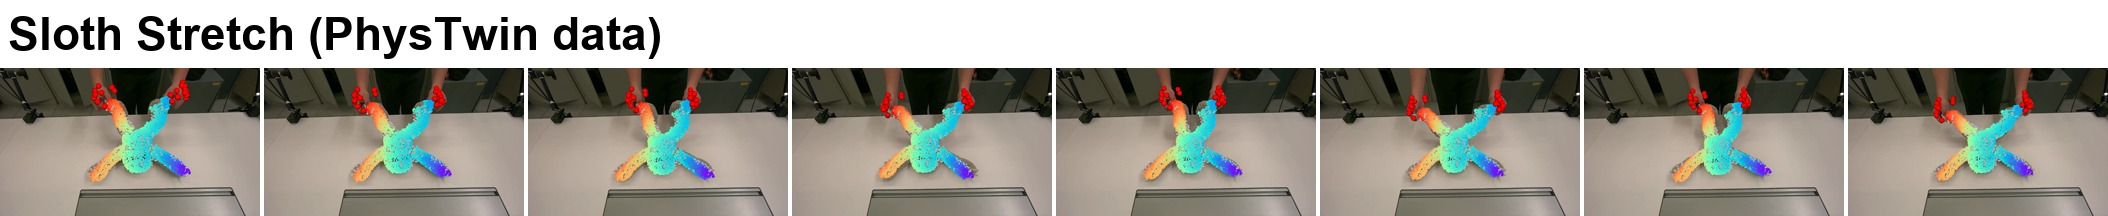
\includegraphics[width = \textwidth]{Images/result_sloth}\\
		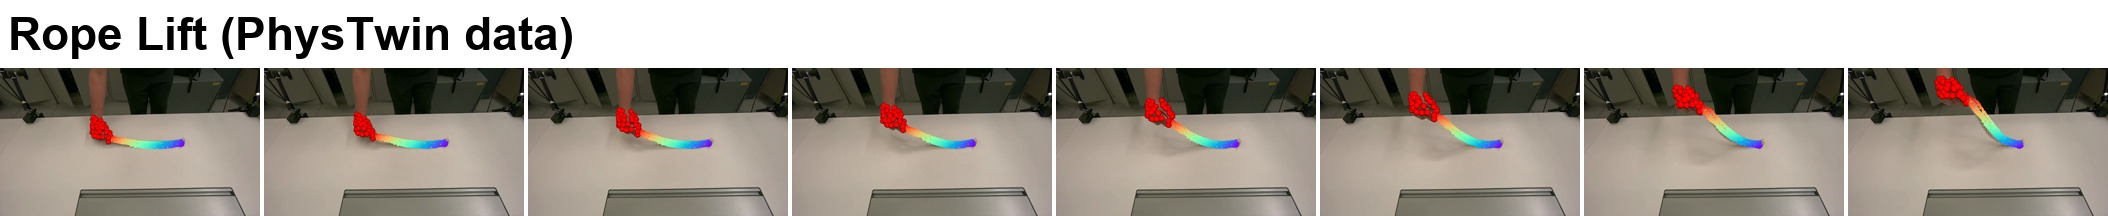
\includegraphics[width = \textwidth]{Images/result_rope}\\
		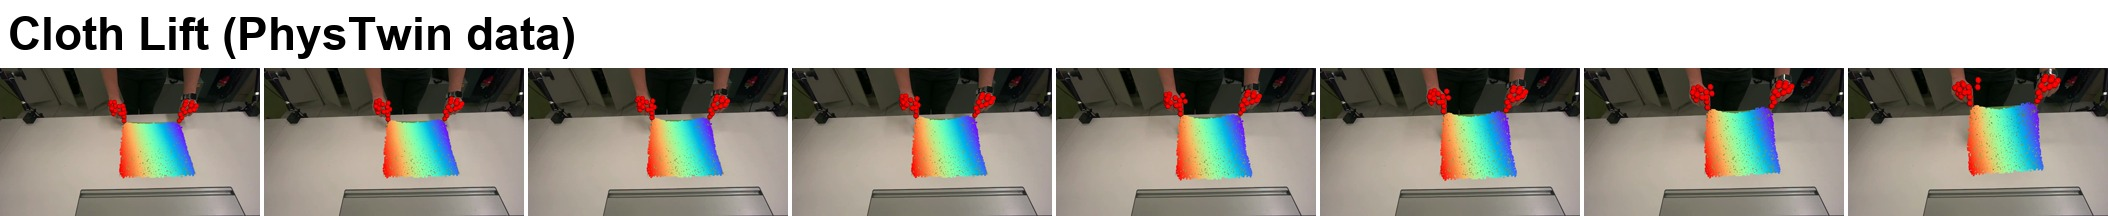
\includegraphics[width = \textwidth]{Images/result_cloth}\\
		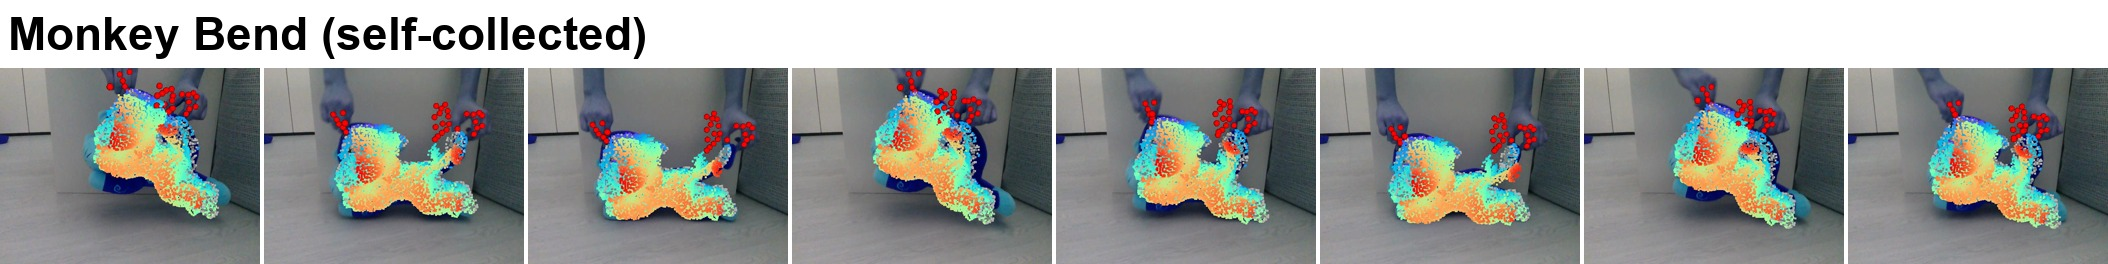
\includegraphics[width = \textwidth]{Images/result_monkey}\\
		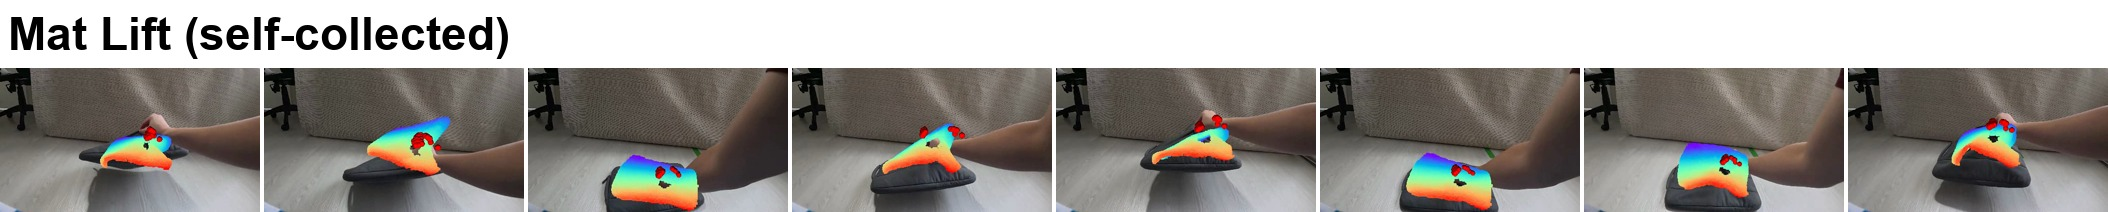
\includegraphics[width = \textwidth]{Images/result_pad}
		\caption{Warp-model results for five objects, eight frames sampled through each clip. Sloth, rope and cloth use PhysTwin data; monkey and mat
		are self-collected.}
		\label{fig:eval-results}
	\end{center}
\end{figure}

Recorded clips of the results are listed in Appendix~\ref{app:results}.

Figure~\ref{fig:eval-results} shows the trained warp models replaying the recorded interactions.
The sloth, cloth and mat rows deform plausibly under the tracked controller motion; the rope row
shows the thin-object case, where the model is driven by few object points. Monkey and mat are
self-collected sessions and complete the pipeline with inferred pose and depth. Mat lift was recorded with looser constraints and still performs reasonably well.

\section{Comparison with the original pipeline}
\label{sec:eval-ognew}

Figure~\ref{fig:eval-ognew} compares the trained warp models of the original PhysTwin pipeline,
which uses the sensor depth, with DIPhysTwin, which uses inferred depth, on the same sequences
and at the same times; Figure~\ref{fig:eval-ognew-2} shows the self-collected monkey and mat sequences. For the monkey and mat pairs, re-captured sessions use recorded depth values, while retraining uses smoothed inferred depth. The
sloth sequence is shown stage by stage in Appendix~\ref{sec:app-vid-sloth-chain}.

\begin{figure}[H]
	\begin{center}
		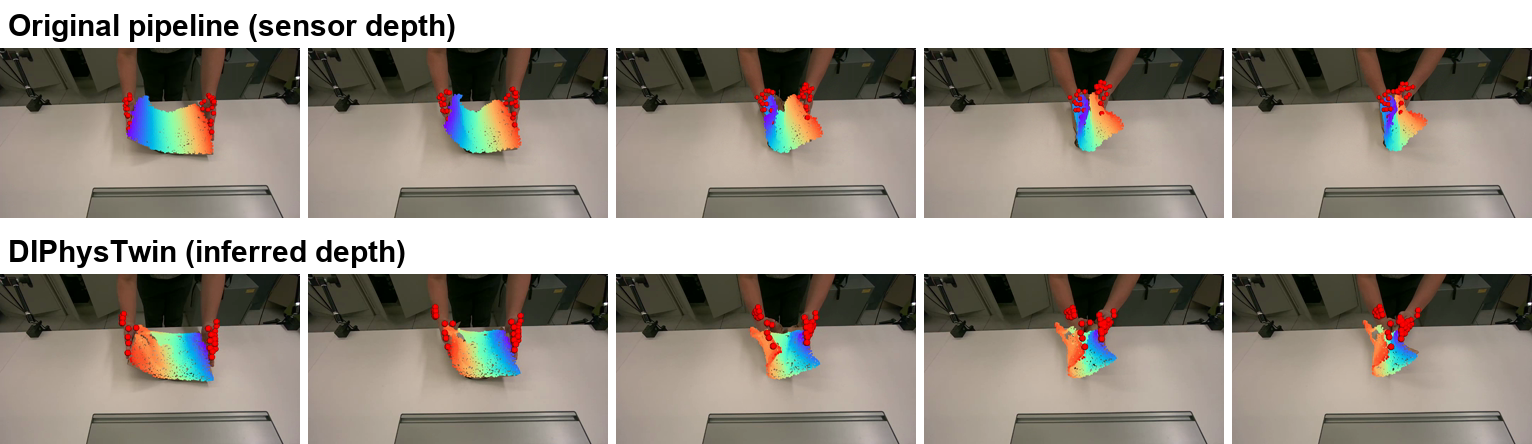
\includegraphics[width = \textwidth]{Images/ognew_package}\\
		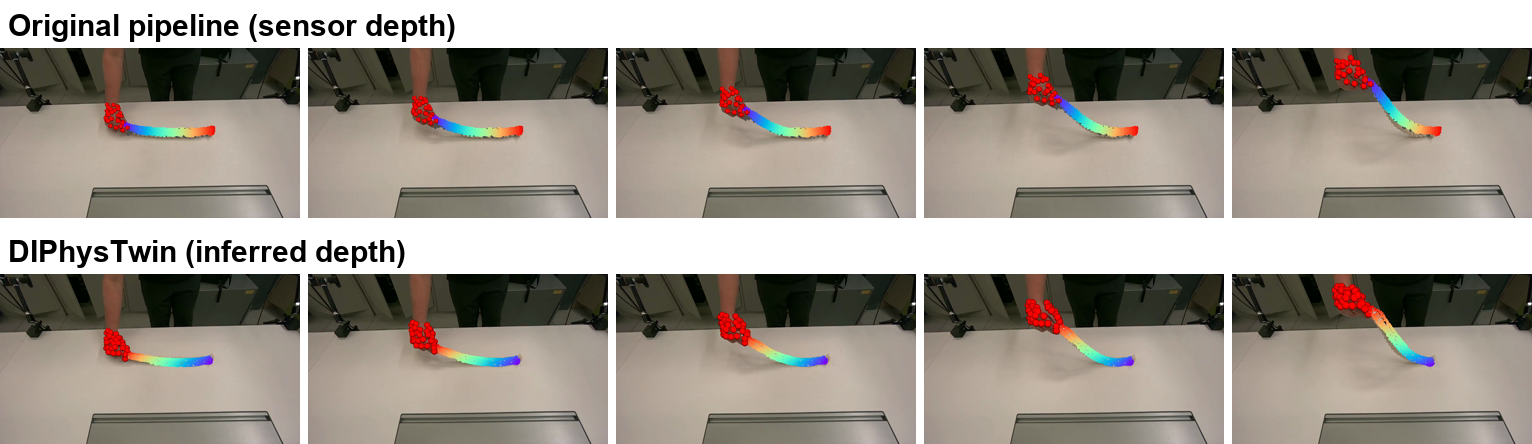
\includegraphics[width = \textwidth]{Images/ognew_rope}\\
		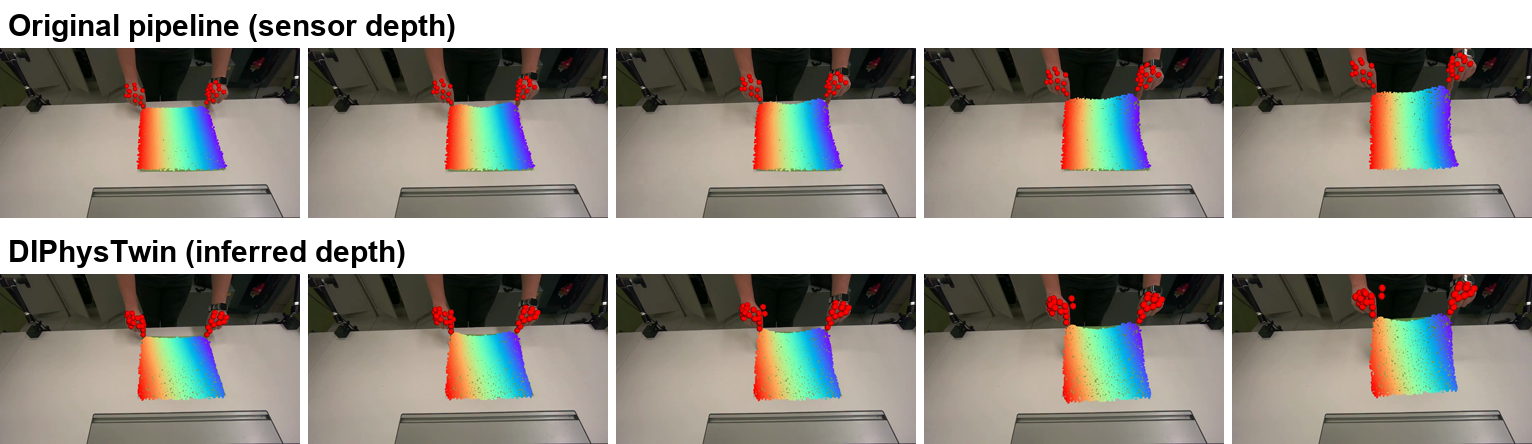
\includegraphics[width = \textwidth]{Images/ognew_cloth}
		\caption{Original PhysTwin pipeline (top row of each object, sensor depth) against
		DIPhysTwin (bottom row, inferred depth) on the package, rope and cloth sequences, at matched
		times.}
		\label{fig:eval-ognew}
	\end{center}
\end{figure}

\begin{figure}[H]
	\begin{center}
		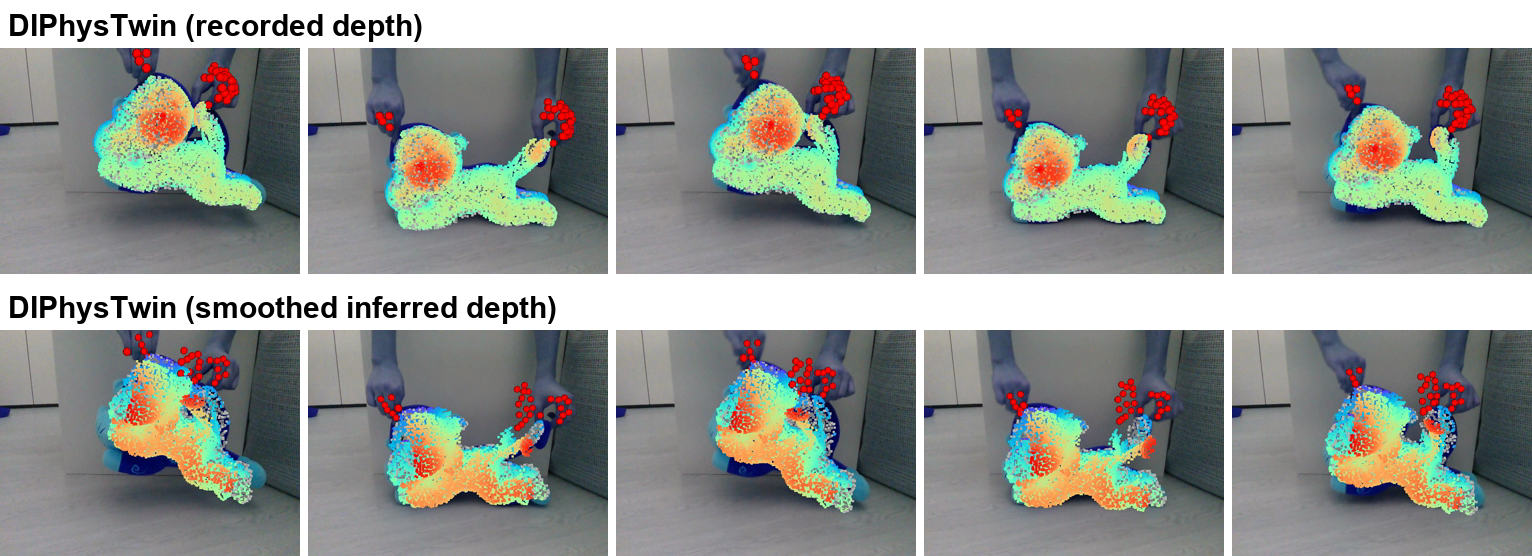
\includegraphics[width = \textwidth]{Images/ognew_monkey}\\
		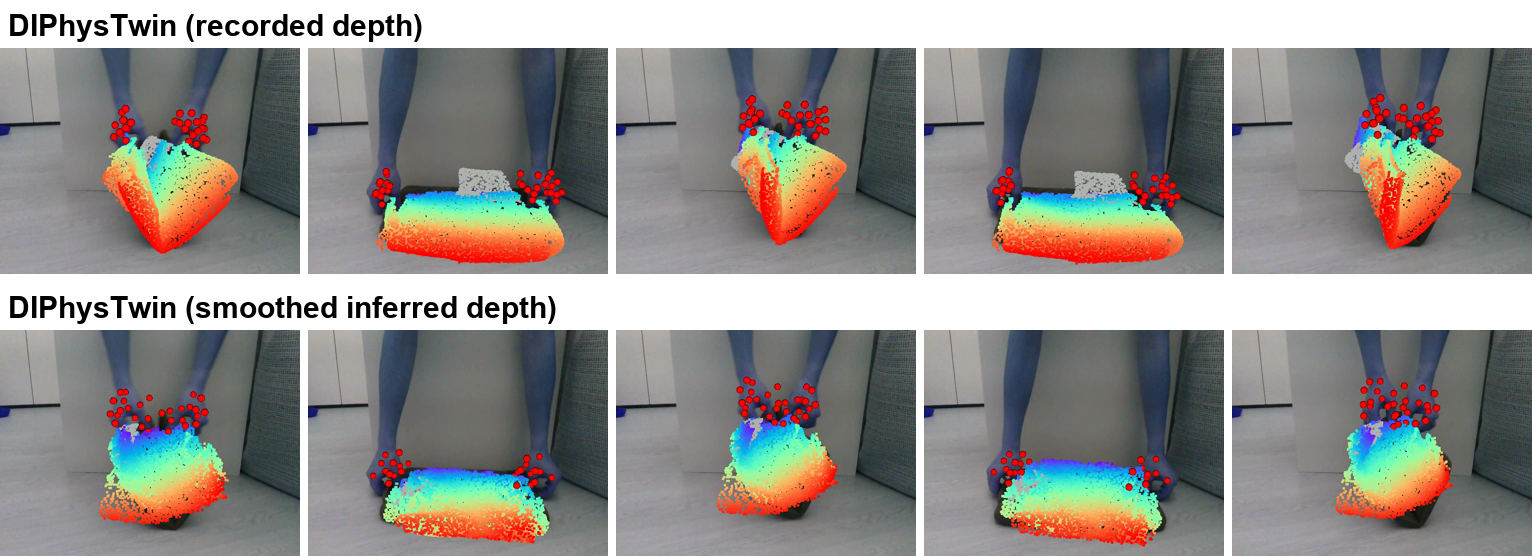
\includegraphics[width = \textwidth]{Images/ognew_pad}
		\caption{The monkey (stuffed animal) and mat sequences. Top row: DIPhysTwin runs with recorded depth; bottom row: runs with smoothed inferred depth.}
		\label{fig:eval-ognew-2}
	\end{center}
\end{figure}

The two rows are hard to compare cleanly. The inferred-depth runs still show jitter and 3D
inconsistency, and these artefacts affect training overall. The two pipelines also differ in other
respects, so the figure does not isolate how much of any difference comes from the depth source alone.

\section{Findings and Failure Cases}
\label{sec:eval-findings}

Large, slow-moving objects with little occlusion reconstructed reliably. Heavy controller
occlusion damaged segmentation, shape-prior generation and tracking. Small, fast-moving objects
showed unstable depth and weaker 3D consistency; recovery also deteriorated when controller contact
was lost. Spatial coherence weakened over time, especially in early unsynchronised captures, and
unusual rotations reconstructed poorly. Soft objects without ground support required excessive
stiffness before ground alignment was corrected; Appendix~\ref{sec:app-vid-ground} shows the rope
sequence before and after the correction.

\begin{table}[H]
	\caption{The author's qualitative assessment of capture conditions and outcome across the self-collected sessions. Outcomes are not counted per session.}
	\label{tab:eval-objects}
	\begin{center}
		\begin{tabular}{@{}>{\raggedright\arraybackslash}p{2.6cm}
		                  >{\raggedright\arraybackslash}p{2.2cm}
		                  >{\raggedright\arraybackslash}p{2.3cm}
		                  >{\raggedright\arraybackslash}p{3.0cm}
		                  >{\raggedright\arraybackslash}p{2.5cm}@{}}
			\toprule
			Object & Scale & Motion speed & Controller occlusion & Outcome \\
			\midrule
			Mat or foam pad & Large & Slow & Minimal & Good \\
			Stuffed animal & Moderate & Slow & Minimal & Good \\
			Cloth & Large & Fast & Significant & Partial \\
			Bottle & Small & Fast & Significant & Poor \\
			Mug & Small & Fast & Significant & Poor \\
			Rope & Large, thin & Slow & None (no ground support) & Partial \\
			\bottomrule
		\end{tabular}
	\end{center}
\end{table}

% The original PhysTwin data is summarised in Table~\ref{tab:phystwin-data} (Chapter~\ref{cha:system-design}).

\section{Negative Results}
\label{sec:eval-negative}

Different tools and methodologies were also tested but did not improve the pipeline. The following list is not exhaustive, but it covers the main alternatives that were tried and abandoned.

Replacing DA3 with $\pi^3$ failed to preserve alignment with known camera poses \parencite{pi3}.
MVTracker performed worse than 2D tracking, while SpatialTrackerV2 produced frequent 3D artefacts
\parencite{mvtracker, spatrackerv2} (Appendix~\ref{sec:app-vid-spatracker}). Trellis and the current CoTracker version gave no
visible improvement \parencite{trellis, cotracker}. Inference without chunk stitching was also tested; its recordings are listed in
Appendix~\ref{sec:app-vid-streaming}.
